\documentclass[a4paper]{article}
\usepackage[margin=1in]{geometry}
\usepackage{hyperref}
\usepackage{graphicx}
%opening
\title{Philosophy of Life Sciences.\\ On Reinfocement Learning and Compatibilism}
\author{Sergei Volodin, EPFL MSc student}
\date{}

\begin{document}

\maketitle

\begin{abstract}
Two seemingly unrelated concepts are considered, namely, Reinfocement Learning and Compatibilism. This paper claims that a new emerging paradigm in Artificial Intelligence, namely, Reinforcement Learning, can answer a question on whether or not free will is compatible with determinism (also known as compatibilism).
First, human behavior are linked with Reinforcement Learning paradigm using recent studies in Computer Science and Neuroscience.
After that, human behavior is analyzed in the RL framework and 
\end{abstract}

\section{Introduction}
Free will is a philosophical concept stating that humans can choose between possible actions in a particular situation \cite{freewillst}.

Reinforcement learning is a subfield of Machine Learning and Artificial Intelligence considering two entities: the {\em agent} and the {\em environment}. {\em Agent} is taking {\em actions} inside the {\em environment}, and the {\em environment} sends this agent back {\em observations}, which are states of the environment and {\em rewards}, which are numbers indicating how well the agent performs \cite{sutton}.

\begin{figure}[h]
	\caption{Reinforcement Learning diagram}
	\centering 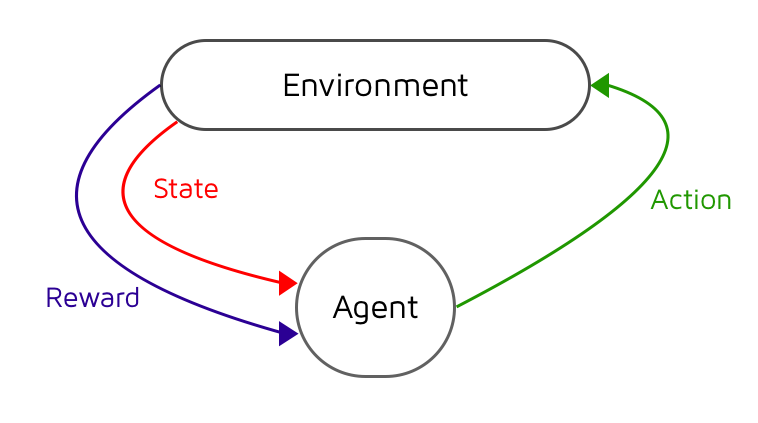
\includegraphics[width=150px]{RL.png}
	\label{RL}
\end{figure}

Recent studies in Neuroscience suggest that the brain of mammals, such as mice and monkeys, uses concepts of Reinforcement Learning in its inner processing to generate action \cite{doyareward, doya2}. Thus, it is plausible to assume that such a framework is also used in humans.

First problem that this essay will address is the seemingly impossible existence of free will under this assumption. If the actions of humans can be explained by a mathematical model, if not in each case, then on average, how can humans might have free will? It shall be shown that reinforcement learning action selection requires randomness in most cases. For example, when choosing exploration or exploitation strategy, most of the agents use a source of random bits. This randomness can come from both of the two entities.

If the randomness comes from the environment, then, in a deterministic world learning would not be possible, meaning that there exist environments for which a randomness-equipped agent can solve, when a deterministic agent cannot.

On the other hand, if the randomness does not come from the environment itself, it can come from inside the agent, meaning that it is the agent who takes decisions of whether or not to explore. This case is exactly considered as free will. It is interpreted as follows: given two equally rewarding options to decide between, $a$ and $b$, and a action-value function $Q(s, a)=Q(s, b)$, the agent himself can choose which action to take, irregardless of the environment, by generating one bit using free will.

However, in this case the environment cannot be deterministic, since human mind is part of it, and it can generate random bits. Thus, we obtain incompatibilism in this case.

Finally, this paper argues that the latter case is true. RL agents and consciousness \cite{rlmorality1}, \cite{rlmorality2}

\begin{thebibliography}{20}
\bibitem{freewillst} \url{https://plato.stanford.edu/entries/freewill/}
\bibitem{doyareward} Kazuyuki Samejima1, Yasumasa Ueda, Kenji Doya1, Minoru Kimura. Representation of Action-Specific Reward Values in the Striatum
\bibitem{doya2} K. Doya. What are the computations of the cerebellum, the basal ganglia and the cerebral cortex?
\bibitem{sutton} Richard S. Sutton and Andrew G. Barto. 1998. Introduction to Reinforcement Learning (1st ed.). MIT Press, Cambridge, MA, USA.
\bibitem{oist} \url{https://groups.oist.jp/ncu} (late 2010s)
\bibitem{freewillrl} Kenneth T. Kishida. A computational approach to “free will” constrained by the games we play
\bibitem{rlmorality1} Brian Tomasik. Do Artificial Reinforcement-Learning Agents Matter Morally?
\bibitem{rlmorality2} \url{http://reducing-suffering.org/ethical-issues-artificial-reinforcement-learning/}
\bibitem{1} \url{http://oxfordindex.oup.com/view/10.1093/acprof:oso/9780198713241.003.0003}
\bibitem{2} Negation of Free will: \url{//www.informationphilosopher.com/freedom/standard_argument.html}
\bibitem{3} \url{https://plato.stanford.edu/entries/freewill/}
\bibitem{4} \url{http://serendip.brynmawr.edu/sci_cult/evolit/s05/web2/lpaterek.html}
\bibitem{5} \url{https://www.researchgate.net/publication/278468286_Creating_Free_Will_in_Artificial_Intelligence}
\bibitem{6} \url{https://philosophy.stackexchange.com/questions/36639/in-what-type-of-world-is-free-will-possible-if-at-all}
\bibitem{7} \url{https://becominghuman.ai/can-a-i-ever-have-free-will-c18b4f489b45}
\bibitem{8} \url{https://philpapers.org/browse/philosophy-of-artificial-intelligence}
\bibitem{9} \url{https://en.wikipedia.org/wiki/Philosophy_of_artificial_intelligence}
\bibitem{a} \url{https://www.theguardian.com/science/2012/oct/03/philosophy-artificial-intelligence}
\bibitem{b} \url{http://jmc.stanford.edu/articles/aiphil2.html}
\bibitem{c} \url{https://plato.stanford.edu/entries/logic-ai/}
\bibitem{d} \url{https://arxiv.org/abs/1605.06048}
\bibitem{e} \url{https://www.youtube.com/watch?v=39EdqUbj92U}
\bibitem{f} \url{https://www.sciencedirect.com/science/article/pii/B9780934613033500337}
\bibitem{g} \url{https://link.springer.com/article/10.1007/s00221-013-3402-y}
\bibitem{h} \url{https://plato.stanford.edu/entries/incompatibilism-theories/}
\bibitem{i} \url{https://github.com/lucasdupin/game_theory_of_life}
\bibitem{j} \url{https://plato.stanford.edu/entries/freewill/}
\bibitem{k} \url{http://andrewmbailey.com/pvi/van_Inwagen_on_Free_Will.pdf}
\bibitem{l} \url{https://www.nature.com/news/2011/110831/full/477023a.html}
\bibitem{m} \url{http://www.sciencedirect.com/science/article/pii/0004370271900117}
\bibitem{n} \url{http://sro.sussex.ac.uk/17112/}
\bibitem{o} \url{https://link.springer.com/book/10.1007\%2F978-3-642-31674-6}
\bibitem{p} \url{https://pdfs.semanticscholar.org/d9f9/91f3a9bc95c9b58dcb8d84aeedb40122ce37.pdf}
\bibitem{q} \url{http://www.sophia.de/pdf/2012_M&M_PT-AI_Introduction.pdf}
\bibitem{r} \url{http://www-formal.stanford.edu/jmc/aiphil.pdf}
\bibitem{s} \url{https://ai.stanford.edu/~nilsson/QAI/qai.pdf}
\bibitem{t} Free will and randomness \url{https://philosophy.stackexchange.com/questions/1012/what-is-the-difference-between-free-will-and-randomness-and-or-non-determinism} \url{https://www.quora.com/What-is-the-difference-between-free-will-and-randomness} \url{https://www.scientificamerican.com/article/quantum-physics-free-will/}
\end{thebibliography}
\end{document}
